\documentclass[../Results.tex]{subfiles}

\begin{document}
	\cite{emonts2019cold} used sensitive low-surface-brightness observations of Very Large Array (VLA) to trace the cold molecular gas in the inner region of MAMMOTH-1 by detecting the CO (1-0) emission. They found four CO sources which are a few kpc away from the associated galaxies or groups. This result suggests that the core of the potential well of this Ly$\alpha$ nebula is marked by the cold gas rather than the obscured AGN. Since none of the continuum image (which center on 35GHz and 150GHz respectively) from VLA and Atacama Large Millimeter/submillimeter Array (ALMA) shows significant detection, we use them to give an 1-$\sigma$ upper limit on its continuum radio emission, $\rm f_{35,up}=0.050$ mJy, $\rm f_{150,up}=0.022$ mJy. By combining these two upper limits with the optical and infrared data from \citet{arrigoni2018overdensity}, we fit the spectral energy distribution (SED) of BOSS1441 and show the result together with M82 template from \cite{Silva_1998} in Fig. \ref{SED}. 
	
	\begin{figure}[htp]
		\centering
		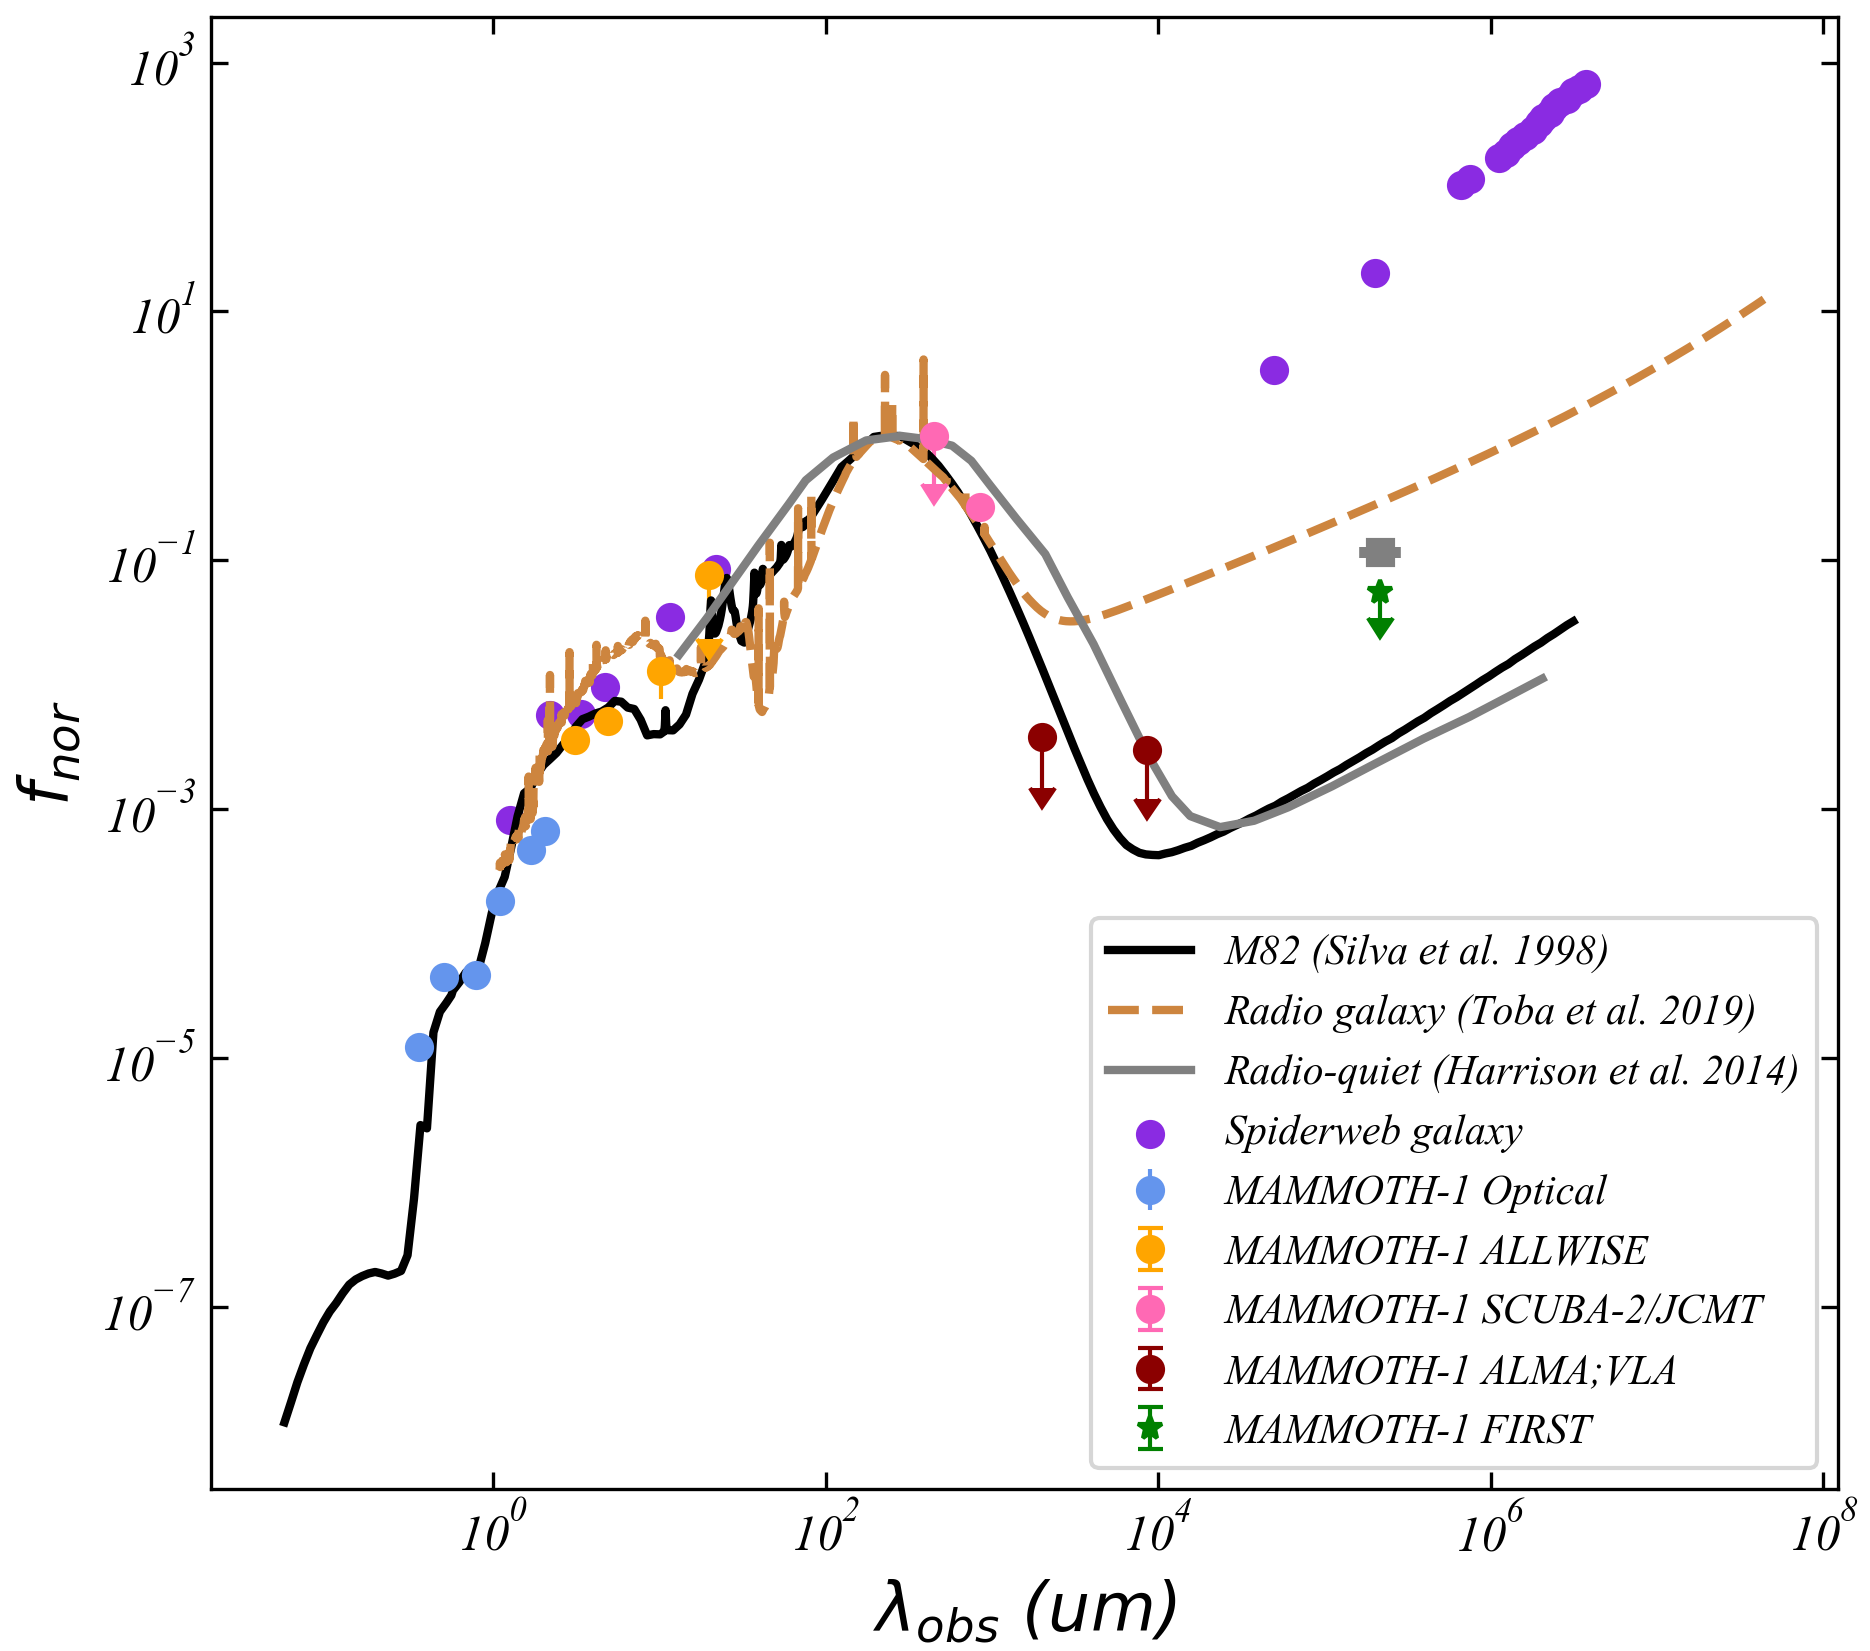
\includegraphics[width=\columnwidth]{figs/SED_fitting}
		\label{SED}
	\end{figure}
	
	We use the definition given by \cite{ivison2010far} to calculate the ratio between the far-infrared ($\rm 8-1000 \ \mu m$) and radio emission ($\rm q_{IR}$), this ratio is usually used to identify if there is significant radio emission above that expected from their star-formation activity (radio emission results from AGN or other process). The formula is given by:
	\begin{equation}
		\rm q_{IR}=log[\frac{S_{IR}/3.75 \times 10^{12} W \ m^{-2}}{S_{1.4}/W \ m^{-2} Hz^{-1}}]
		\label{q_IR}
	\end{equation}
	where $\rm S_{IR}$ is the rest-frame flux in far-infrared range ($8-1000 \ \rm \mu m $) and $\rm S_{1.4}$ is the rest-frame 1.4 GHz flux density. \citep{arrigoni2018overdensity} performed a follow-up observation for MAMMOTH-1 and constrain the SED with the available data. They found the SED of local starburst galaxy M82 match significantly well with the observations which indicates that BOSS1441 is possibly an Ultra-Luminous Infrared Galaxy (ULIG). The far-infrared luminosity is then integrated from this SED $\rm L_{IR}=3.2 \times 10^{12}L_{\odot}$. Through setting the luminosity distance to be $\rm D_{L}=18773.8$ Mpc at redshift z=2.3, it is easy to calculate the far-infrared flux $\rm S_{IR}=2.9 \times 10^{-16}\ W \ cm^{-2}$.  Because the D-configuration of VLA doesn't cover $\rm \nu_{obs}=0.42$ GHz (1.4 GHz in rest frame), we adopt $\rm S_{1.4}$=0.01 mJy from M82 SED template. We note here that the constrain of continuum, $f_{150,up}$, is one-order-magnitude lower than that of M82 SED template, therefore the true flux density at $\rm \nu_{rest}=1.4$GHz should be lower than 0.01 mJy. By adopting $\rm S_{1.4}=0.01 mJy$ the low limit of $\rm q_{IR}$ is equal to 1.9. \cite{ivison2010far} and \cite{del2013goods} define "radio excess" sources as those with $\rm q_{IR} \leqslant 1.8$, according to this definition and $\rm q_{IR}$ calculated here, we suggest BOSS1441 is a radio-quiet source with no significant continuum radio emission.
\end{document}